 \chapterhead{CHƯƠNG 1 $-$ TỔNG QUAN VỀ VPN}
    \addcontentsline{toc}{chapter}{CHƯƠNG 1 $-$ TỔNG QUAN VỀ VPN}
    \section*{1.1 Giới thiệu}
    \addcontentsline{toc}{section}{1.1 Giới thiệu}
    Trong kỷ nguyên số, Internet đã trở thành một phần không thể thiếu trong cuộc sống của chúng ta. Với khả năng kết nối mọi người và mọi thứ trên toàn cầu, Internet đã tạo ra những cơ hội kinh doanh mới, thúc đẩy sự phát triển của nền kinh tế. Tuy nhiên, bên cạnh những lợi ích to lớn, Internet cũng đặt ra nhiều thách thức về bảo mật và an toàn thông tin, đặc biệt là khi các cuộc tấn công mạng ngày càng trở nên tinh vi. Để giải quyết vấn đề này, mạng riêng ảo (VPN) đã ra đời, cung cấp một giải pháp an toàn và hiệu quả để bảo vệ dữ liệu và đảm bảo kết nối riêng tư trên mạng công cộng.

    VPN không chỉ đơn thuần là một công cụ để bảo vệ dữ liệu, mà còn là một công cụ để mở rộng khả năng kết nối của người dùng. Ví dụ, một du khách đi du lịch nước ngoài có thể sử dụng VPN để truy cập vào các dịch vụ ngân hàng trực tuyến của nước mình một cách an toàn, kể cả mạng Wi-Fi công cộng không được bảo mật.
    \begin{figure}[htbp]
        \centering
        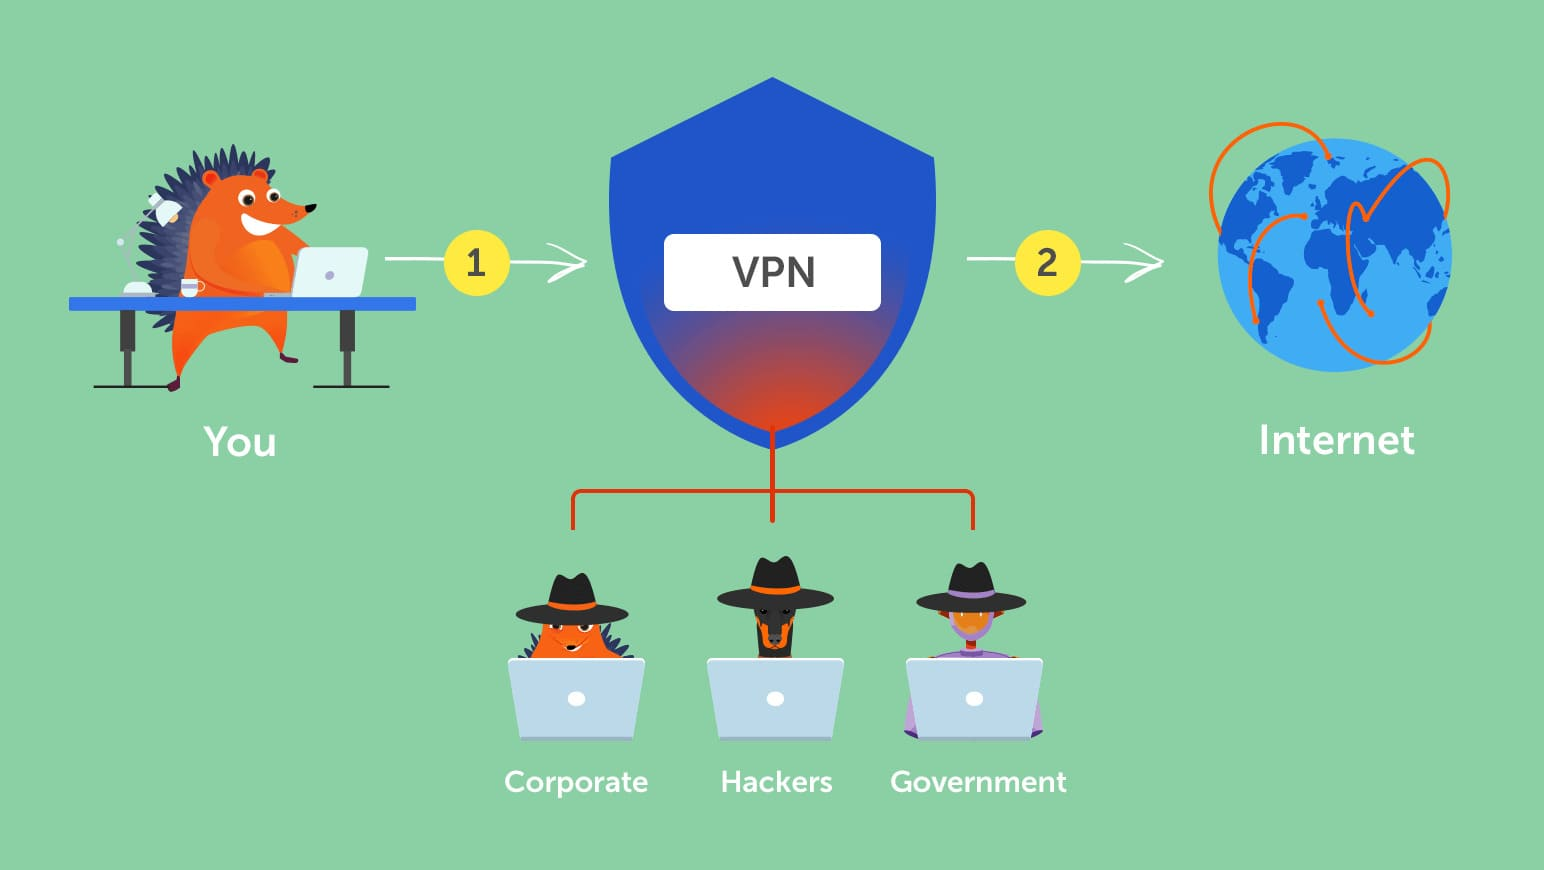
\includegraphics[width=0.7\linewidth]{img/whatvpn.png}
        \caption{VPN là gì}
    \end{figure}
    
    Do đó, VPN đã và đang trở thành một công cụ không thể thiếu trong việc bảo vệ thông tin cá nhân và doanh nghiệp. Với khả năng mã hóa dữ liệu, ấn danh hoạt động trực tuyến và cho phép truy cập an toàn mạng nội bộ, VPN đã giải quyết được những thách thức mà Internet đã đặt ra. Chắc chắn, trong tương lai VPN sẽ ngày càng trở nên phổ biến và được tích hợp vào nhiều dịch vụ và thiết bị khác nhau, mang đến cho người dùng trải nghiệm trực tuyến an toàn và bảo mật hơn. Trong nhiều trường hợp VPN cũng giống như WAN, tuy nhiên đặc tính quyết định của VPN là chúng có thể dùng mạng công cộng như Internet mà đảm bảo tính riêng tư và tiết kiệm hơn nhiều.
    \subsection*{1.1.1 Định nghĩa VPN}
    \addcontentsline{toc}{subsection}{1.1.1 Định nghĩa VPN}
    VPN là viết tắt của \textit{Virtual Private Network}, còn được gọi là mạng riêng ảo, là phương pháp làm cho mạng công cộng được hoạt động như một mạng LAN nhưng được phát triển và mở rộng hơn. VPN cho phép thiết lập các kết nối riêng với những người dùng ở xa, các văn phòng chi nhánh của công ty và đối tác của công ty đang sử dụng chung một đường mạng công cộng.
    \begin{figure}[htbp]
        \centeringơ
        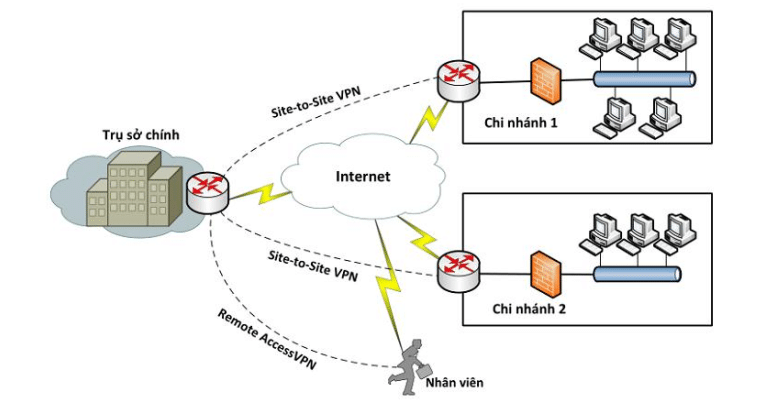
\includegraphics[width=0.7\linewidth]{img/vpnmodel.png}
        \caption{Mô hình VPN}
    \end{figure}
    
    Về cơ bản, VPN là một mạng riêng sử dụng hệ thống mạng công cộng (thường là Internet) để kết nối các địa điểm hoặc người sử dụng từ xa. Thay vì dùng kết nối thật khá phức tạp như đường dây số thuê bao, VPN tạo ra các liên kết ảo được truyền qua Internet giữa mạng riêng của tổ chức với địa điểm người sử dụng ở xa. Ngoài ra, ở mạng WAN yêu cầu công ty phải trả chi phí để duy trì nhiều loại đường dây riêng, trong khi đó, VPN không bị ảnh hưởng bởi chi phí như WAN do thực hiện qua một mạng công cộng.

    Để có thể gửi và nhận dữ liệu thông qua mạng công cộng mà vẫn đảm bảo tính an toàn, bảo mật thì VPN cung cấp các cơ chế mã hóa dữ liệu trên đường truyền tạo ra một "đường hầm" bảo mật giữa nơi nhận và nơi gửi (Tunnel), giống như kết nối point-to-point trên mạng riêng. Để tạo ra một "đường hầm" bảo mật đó, dữ liệu được mã hóa chỉ cung cấp phần đầu của gói dữ liệu là thông tin về quãng đường đi, cho phép nó có thể di chuyển nhanh chóng thông qua mạng công cộng. Dữ liệu được mã hóa một cách cẩn thận, do đó nếu các packet bị bắt lại trên đường truyền công cộng cũng không thể đọc được nội dung vì không có khóa để giải mã.

    Có thể xem VPN là một giải pháp được thiết kế dành cho các tổ chức, doanh nghiệp có xu hướng tăng cường thông tin từ xa vì địa bàn hoạt động rộng (trên toàn quốc hay toàn cầu), vừa an toàn, vừa tiết kiệm chi phí và thời gian.
    \subsection*{1.1.2 Lợi ích của VPN}
    \addcontentsline{toc}{subsection}{1.1.2 Lợi ích của VPN}

    VPN mang lại nhiều lợi ích đáng kể cho người dùng Internet. Dưới đây là một số lợi ích chính mà VPN đem lại cho người sử dụng:

    $-$ Bảo mật thông tin cá nhân cho người dùng:
    \begin{itemize}
        \item \textit{Mã hóa dữ liệu}: Mã hóa dữ liệu giúp bảo vệ thông tin cá nhân khỏi bị theo dõi hoặc đánh cắp, đặc biệt khi sử dụng mạng Wi-Fi công cộng.
        \item \textit{Ẩn địa chỉ IP}: VPN thay thế địa chỉ IP thực bằng một địa chỉ IP khác, khiến việc theo dõi hoạt động trực tuyến trở nên khó khăn hơn.
    \end{itemize}

    $-$ Truy cập được các nội dung bị hạn chế:
    \begin{itemize}
        \item \textit{Vượt qua tường lửa}: VPN cho phép kết nối, truy cập an toàn các trang web và dịch vụ bị chặn ở một số quốc gia hoặc mạng nội bộ.
    \end{itemize}

    $-$ Tăng cường quyền riêng tư:
    \begin{itemize}
        \item \textit{Ngăn chặn theo dõi}: VPN giúp ngăn chặn các nhà cung cấp dịch vụ Internet, nhà quảng cáo và các bên thứ ba theo dõi hoạt động trực tuyến.
        \item \textit{Bảo vệ danh tính}: VPN bảo vệ danh tính người dùng khi đang sử dụng các mạng công cộng.
    \end{itemize}

    $-$ An toàn khi làm việc từ xa:
    \begin{itemize}
        \item \textit{Kết nối mạng công ty an toàn}: VPN tạo ra một đường hầm an toàn để kết nối thiết bị người sử dụng với mạng công ty, cho phép làm việc từ xa một cách bảo mật bất cứ lúc nào. $=>$ Năng suất làm việc được nâng cao.
    \end{itemize}
    \section*{1.2 Phân loại VPN}
    \addcontentsline{toc}{section}{1.2 Phân loại VPN}
    VPN là khái niệm chung cho việc thiết lập kênh truyền ảo, nhưng còn tùy thuộc vào mô hình mạng và nhu cầu sử dụng mà chọn loại thiết kế cho phù hợp. Công nghệ VPN có thể được phân thành 2 loại cơ bản: Site-to-Site VPN và Remote Access VPN.
    \subsection*{1.2.1 Remote Access VPN}
    \addcontentsline{toc}{subsection}{1.2.1 Remote Access VPN}
    
    Remote Access VPN còn có thể hiểu là mô hình Client-to-site, cho phép truy cập bất cứ lúc nào bằng Remote, Mobile, và các thiết bị truyền thông của nhân viên các chi nhánh kết nối đến tài nguyên của tổ chức. Đảm bảo tính bảo mật của dữ liệu và tài nguyên mạng nội bộ khi nhân viên truy cập từ xa, ngay cả khi họ sử dụng mạng công cộng không an toàn.

    \begin{figure}[htbp]
        \centering
        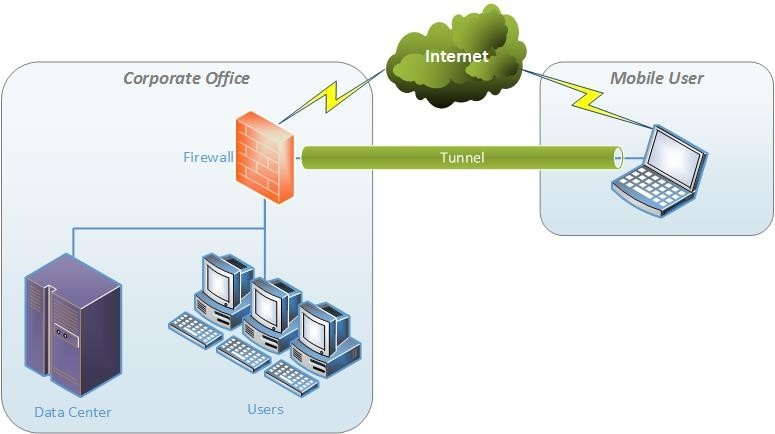
\includegraphics[width=0.5\linewidth]{img/remote.png}
        \caption{Mô hình Remote Access VPN}
    \end{figure}

    Thông tin của người dùng và dữ liệu truyền tải sẽ được mã hoá hoàn toàn khi kết nối thông qua mạng công cộng. Vì thế mà giảm thiểu tối đa rủi ro các hình thức tấn công không gian mạng. Loại mô hình này thường được áp dụng cho nhân viên làm việc lưu động hay làm việc tại nhà muốn kết nối vào mạng công ty an toàn.

    \begin{figure}[htbp]
        \centering
        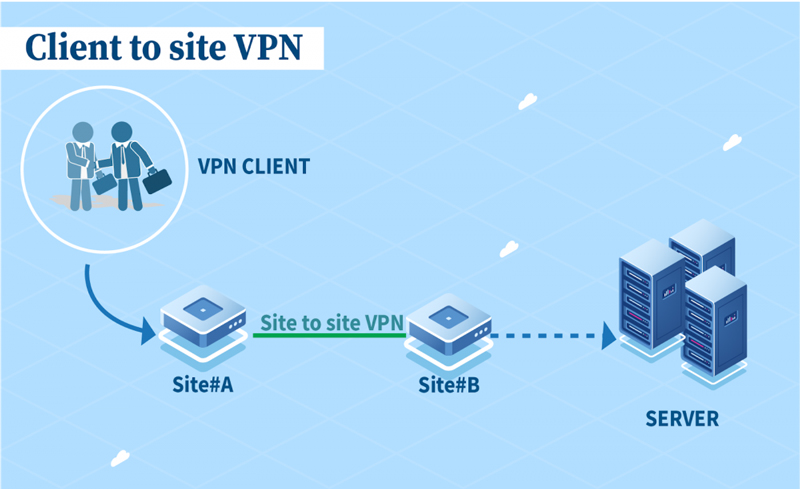
\includegraphics[width=0.7\linewidth]{img/vpn-client-to-site.jpeg}
        \caption{Remote Access kết nối người dùng đến mạng công ty}
    \end{figure}

    Một hướng phát triển mới trong Remote Access VPN là dùng Wireless VPN, trong đó một nhân viên có thể truy cập mạng của họ thông qua kết nối không dây. Trong thiết kế này, các kết nối không dây cần phải kết nối về một trạm Wireless (Wireless Terminal) và sau đó về mạng của công ty. Trong cả hai trường hợp, phần mềm client trên máy PC đều cho phép khởi tạo các kết nối bảo mật, còn được gọi là tunnel.
    
    \subsection*{1.2.2 Site-to-site VPN}
    \addcontentsline{toc}{subsection}{1.2.2 Site-to-site VPN}

    Site to site VPN là mô hình dùng để kết nối các hệ thống mạng ở các nơi khác nhau tạo thành một hệ thống mạng thống nhất. Ở loại kết nối này thì việc chứng thực ban đầu phụ thuộc vào thiết bị đầu cuối ở các Site, các thiết bị này hoạt động như Gateway và đây là nơi đặt nhiều chính sách bảo mật nhằm truyền dữ liệu một cách an toàn giữa các Site. Mô hình này thường được triển khai trên mạng có băng thông cao và đáng tin cậy cho phép truyền tải dữ liệu lớn và đảm bảo hiệu suất ổn định cho các ứng dụng quan trọng của tổ chức.
    \begin{figure}[htbp]
        \centering
        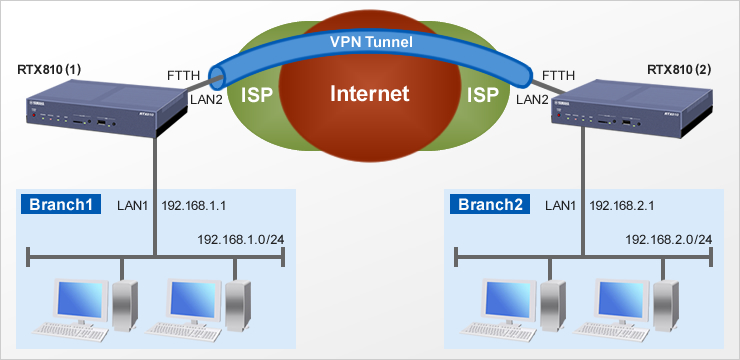
\includegraphics[width=0.6\linewidth]{img/Sitetosite.png}
        \caption{Mô hình Site-to-site VPN}
    \end{figure}


    Mô hình VPN này là sự kết nối hai mạng riêng lẻ thông qua một đường hầm bảo mật, đường hầm bảo mật này có thể sử dụng các giao thức PPTP, L2TP, hoặc IPSec, mục đích của Site –to –Site VPN là kết nối hại mạng không có đường nối lại với nhau, không có việc thoả hiệp tích hợp, chứng thực, sự cẩn mật của dữ liệu, có thể thiết lập một Site – to –Site VPN thông qua sự kết hợp của các thiết bị VPN concentrators, Router, và Firewalls.

    VPN site-to-site được sử dụng khi muốn kết nối các chi nhánh, văn phòng của công ty với nhau (Intranet VPN) hoặc kết nối với công ty đối tác (Extranet VPN). Lúc này, mọi nhân viên, thiết bị ở cả các địa điểm có thể trao đổi mọi thông tin với nhau thông qua kết nối VPN.

    \begin{figure}[htbp]
        \centering
        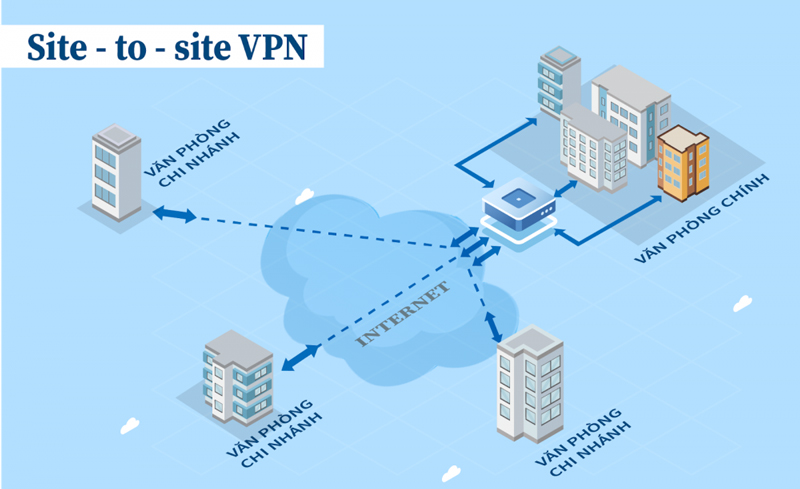
\includegraphics[width=0.6\linewidth]{img/vpn-site-to-site.jpeg}
        \caption{Site-to-site kết nối các chi nhánh}
    \end{figure}

    
    \section*{1.3 Ưu nhược điểm của VPN}
    \addcontentsline{toc}{section}{1.3 Ưu nhược điểm của VPN}
    \subsection*{1.3.1 Ưu điểm}
    \addcontentsline{toc}{subsection}{1.3.1 Ưu điểm}

    Mạng riêng ảo có nhiều ưu điểm thực sự và tức thời cho các công ty, tổ chức, giúp đơn giản hoá việc trao đổi thông tin giữa các nhân viên làm việc ở xa, người dùng lưu động,...
    \begin{itemize}
        \item \textit{Tiết kiệm chi phí}: Thay vì đầu tư vào các đường truyền riêng đắt tiền, VPN tận dụng mạng Internet công cộng hiện có, vì thế mà có thể tiết kiệm đáng kể chi phí ban đầu và chi phí vận hành. Nhiều số liệu cho thấy, giá thành cho việc kết nối LAN-to-WAN giảm từ 20\% - 30\% so với việc sử dụng đường thuê riêng truyền thống, còn với việc truy cập từ xa giảm từ 60\% - 80\%.
        \item \textit{Tính linh hoạt}: Tính linh hoạt không chỉ bao gồm việc truy cập từ mọi nơi, mà VPN còn linh hoạt trọng việc hỗ trợ nhiều thiết bị, tích hợp các ứng dụng. VPN có thể được cài trên máy tính, điện thoại, máy tính bảng giúp người dùng dễ dàng kết nối bất kì lúc nào, do đó cũng giúp tạo ra một môi trường làm việc liền mạch và hiệu quả.
        \item \textit{Khả năng mở rộng}: Do sử dụng mạng công cộng nên bất cứ ở nơi nào có Internet đều có thể triển khai VPN. Dễ dàng mở rộng băng thông hay gỡ bỏ VPN khi không còn nhu cầu sử dụng. Điều này đáp ứng được nhu cầu tăng trưởng của doanh nghiệp mà không cần phải đầu tư quá nhiều vào hạ tầng.
        \item \textit{Giảm thiểu các hỗ trợ kỹ thuật}: Việc kết nối từ xa đã giảm thiểu các vấn đề kỹ thuật phát sinh và đơn giản hoá quá trình hổ trợ người dùng. Ngoài ra, việc chuẩn hoá trên một kiểu kết nối đối tượng di động đến một POP của ISP và chuẩn hoá các yêu cầu bảo mật cũng làm giảm thiểu nhu cầu về nguồn hỗ trợ kỹ thuật của VPN.
        \item \textit{Giảm thiểu các yêu cầu về thiết bị}: VPN tận dụng hạ tầng mạng hiện có, giảm thiểu nhu cầu đầu tư vào các thiết bị mạng chuyên dụng như router, firewall. Do giảm thiểu số lượng thiết bị mạng nên tiết kiệm không gian và năng lượng. 
        \item \textit{Đáp ứng nhu cầu thương mại}: Triển khai mô hình VPN giúp thương hiệu, uy tín của doanh nghiệp được đảm bảo an toàn và tuân thủ các quy định về bảo mật dữ liệu cho khách hàng, tránh các rủi ro pháp lý. Bên cạnh đó, VPN tạo điều kiện thuận lợi cho việc hợp tác với đối tác kinh doanh ở xa, giúp tăng cường hiệu quả làm việc và thị trường được mở rộng.
    \end{itemize}
    
    \subsection*{1.3.2 Nhược điểm}
    \addcontentsline{toc}{subsection}{1.3.2 Nhược điểm}

    Bên cạnh những ưu điểm nổi bật trong việc triển khai mô hình VPN, để đánh giá một cách toàn diện về VPN thì không thể bỏ qua những hạn chế nhất định.
    \begin{itemize}
        \item \textit{Phụ thuộc nhiều vào chất lượng của mạng Internet}: Do có thể kết nối từ bất kì nơi nào có Internet nên VPN phụ thuộc nhiều vào chất lượng mạng như tốc độ kết nối, độ trễ, mất gói tin,...Sự quá tải hay tắc nghẽn mạng sẽ làm ảnh hưởng đến chất lượng truyền thông tin.
        \item \textit{Thiếu các giao thức kế thừa hỗ trợ}: Không phải tất cả các thiết bị và ứng dụng đều hỗ trợ đầy đủ các giao thức VPN hiện đại. Điều này đã gây ra khó khăn trong việc thiết lập và cấu hình VPN, đặc biệt là đối với hệ thống cũ và các ứng dụng chuyên dụng. Không chỉ bị hạn chế về khả năng tương thích, mà một số giao thức VPN cũ có thể không hỗ trợ các tính năng tiên tiến như mã hoá mạnh, xác thực hai yếu tố, làm giảm khả năng bảo mật và quản lý của VPN.
        \item \textit{Vấn đề an ninh}: Mặc dù được thiết kế để ẩn địa chỉ IP, nhưng nếu không được cấu hình đúng cách, DNS có thể bị rò rỉ làm lộ thông tin về các trang web mà người dùng truy cập. Ngoài ra, cấu hình sai có thể dẫn đến các lỗ hỏng bảo mật, khiến tin tặc dễ xâm nhập vào hệ thống và khai thác dữ liệu của doanh nghiệp.
        \item \textit{Độ tin cậy và thực thi}: VPN có thể bị các nhà cung cấp dịch vụ ISP hoặc các trang web phát hiện và chặn, làm giảm hiệu quả sử dụng VPN.
    \end{itemize}
  
    